\documentclass{beamer}

\usepackage[T1, T2A]{fontenc}
\usepackage[utf8]{inputenc}
\usepackage[english, russian]{babel}

\usetheme{Madrid}
\usecolortheme{beaver}
\setbeamertemplate{caption}[numbered]
\makeatother
\setbeamertemplate{footline}
{\leavevmode%
  \hbox{%
  \begin{beamercolorbox}[wd=.4\paperwidth,ht=2.25ex,dp=1ex,center]{author in head/foot}%
      \usebeamerfont{author in head/foot}\insertshortauthor{}~(\insertshortinstitute{})
  \end{beamercolorbox}%
  \begin{beamercolorbox}[wd=.5\paperwidth,ht=2.25ex,dp=1ex,center]{title in head/foot}%
    \usebeamerfont{title in head/foot}\insertshorttitle
  \end{beamercolorbox}%
  \begin{beamercolorbox}[wd=.1\paperwidth,ht=2.25ex,dp=1ex,center]{date in head/foot}%
    \insertframenumber{} / \inserttotalframenumber\hspace*{1ex}
  \end{beamercolorbox}}%
}
\makeatletter
\setbeamertemplate{navigation symbols}{}

\usepackage{animate}
\usepackage{graphicx}
\bibliographystyle{unsrt}

\usepackage{hyperref}
\hypersetup{colorlinks=true,
    linkcolor=blue,
    filecolor=magenta,
    urlcolor=cyan,
}

\usepackage{amssymb}
\usepackage{amsmath}
\usepackage{amsthm}
\usepackage{lscape}
\usepackage{color}
\graphicspath{{./images/}}

\AtBeginSection[]
{
    \begin{frame}
        \frametitle{Содержание}
        \tableofcontents[currentsection]
    \end{frame}
}

\title[3D реконструкция поверхности в СЭМ]{Трехмерная сканирующая электронная микроскопия
топографии поверхности с учетом влияния функции отклика детекторной системы:
математические методы обработки данных.}
\author[А.А.~Борзунов]{А.А.~Борзунов\inst{1} \and Д.В.~Лукьяненко\inst{1} \and Э.И.~Рау \inst{1} \and А.Г.~Ягола \inst{1}}
\institute[МГУ им. М.В. Ломоносова]{Московский Государственный Университет им. М.В. Ломоносова}
\titlegraphic{\includegraphics[width=2cm]{ff.png}}

\date{21 Апреля 2021 г.}



\begin{document}

\begin{frame}
    \titlepage
\end{frame}

%---------------------------------------------------------------------------------------------------

\section{Проблематика}
\begin{frame}
    \sectionpage
\end{frame}

\begin{frame}[c]
    \frametitle{Проблематика}
    \begin{columns}
        \begin{column}{0.5\textwidth}
            \includegraphics[width=1.0\linewidth]{VA.png}
        \end{column}
        \begin{column}{0.5\textwidth}
            % nothing here, will be in the next frame
        \end{column}
    \end{columns}
\end{frame}

% Создаем анимацию посредством копирования слайда :-)
\begin{frame}[c]
    \frametitle{Проблематика}
    \begin{columns}
        \begin{column}{0.38\textwidth}
            \includegraphics[width=1.0\linewidth]{VA.png}
        \end{column}
        \begin{column}{0.58\textwidth}
            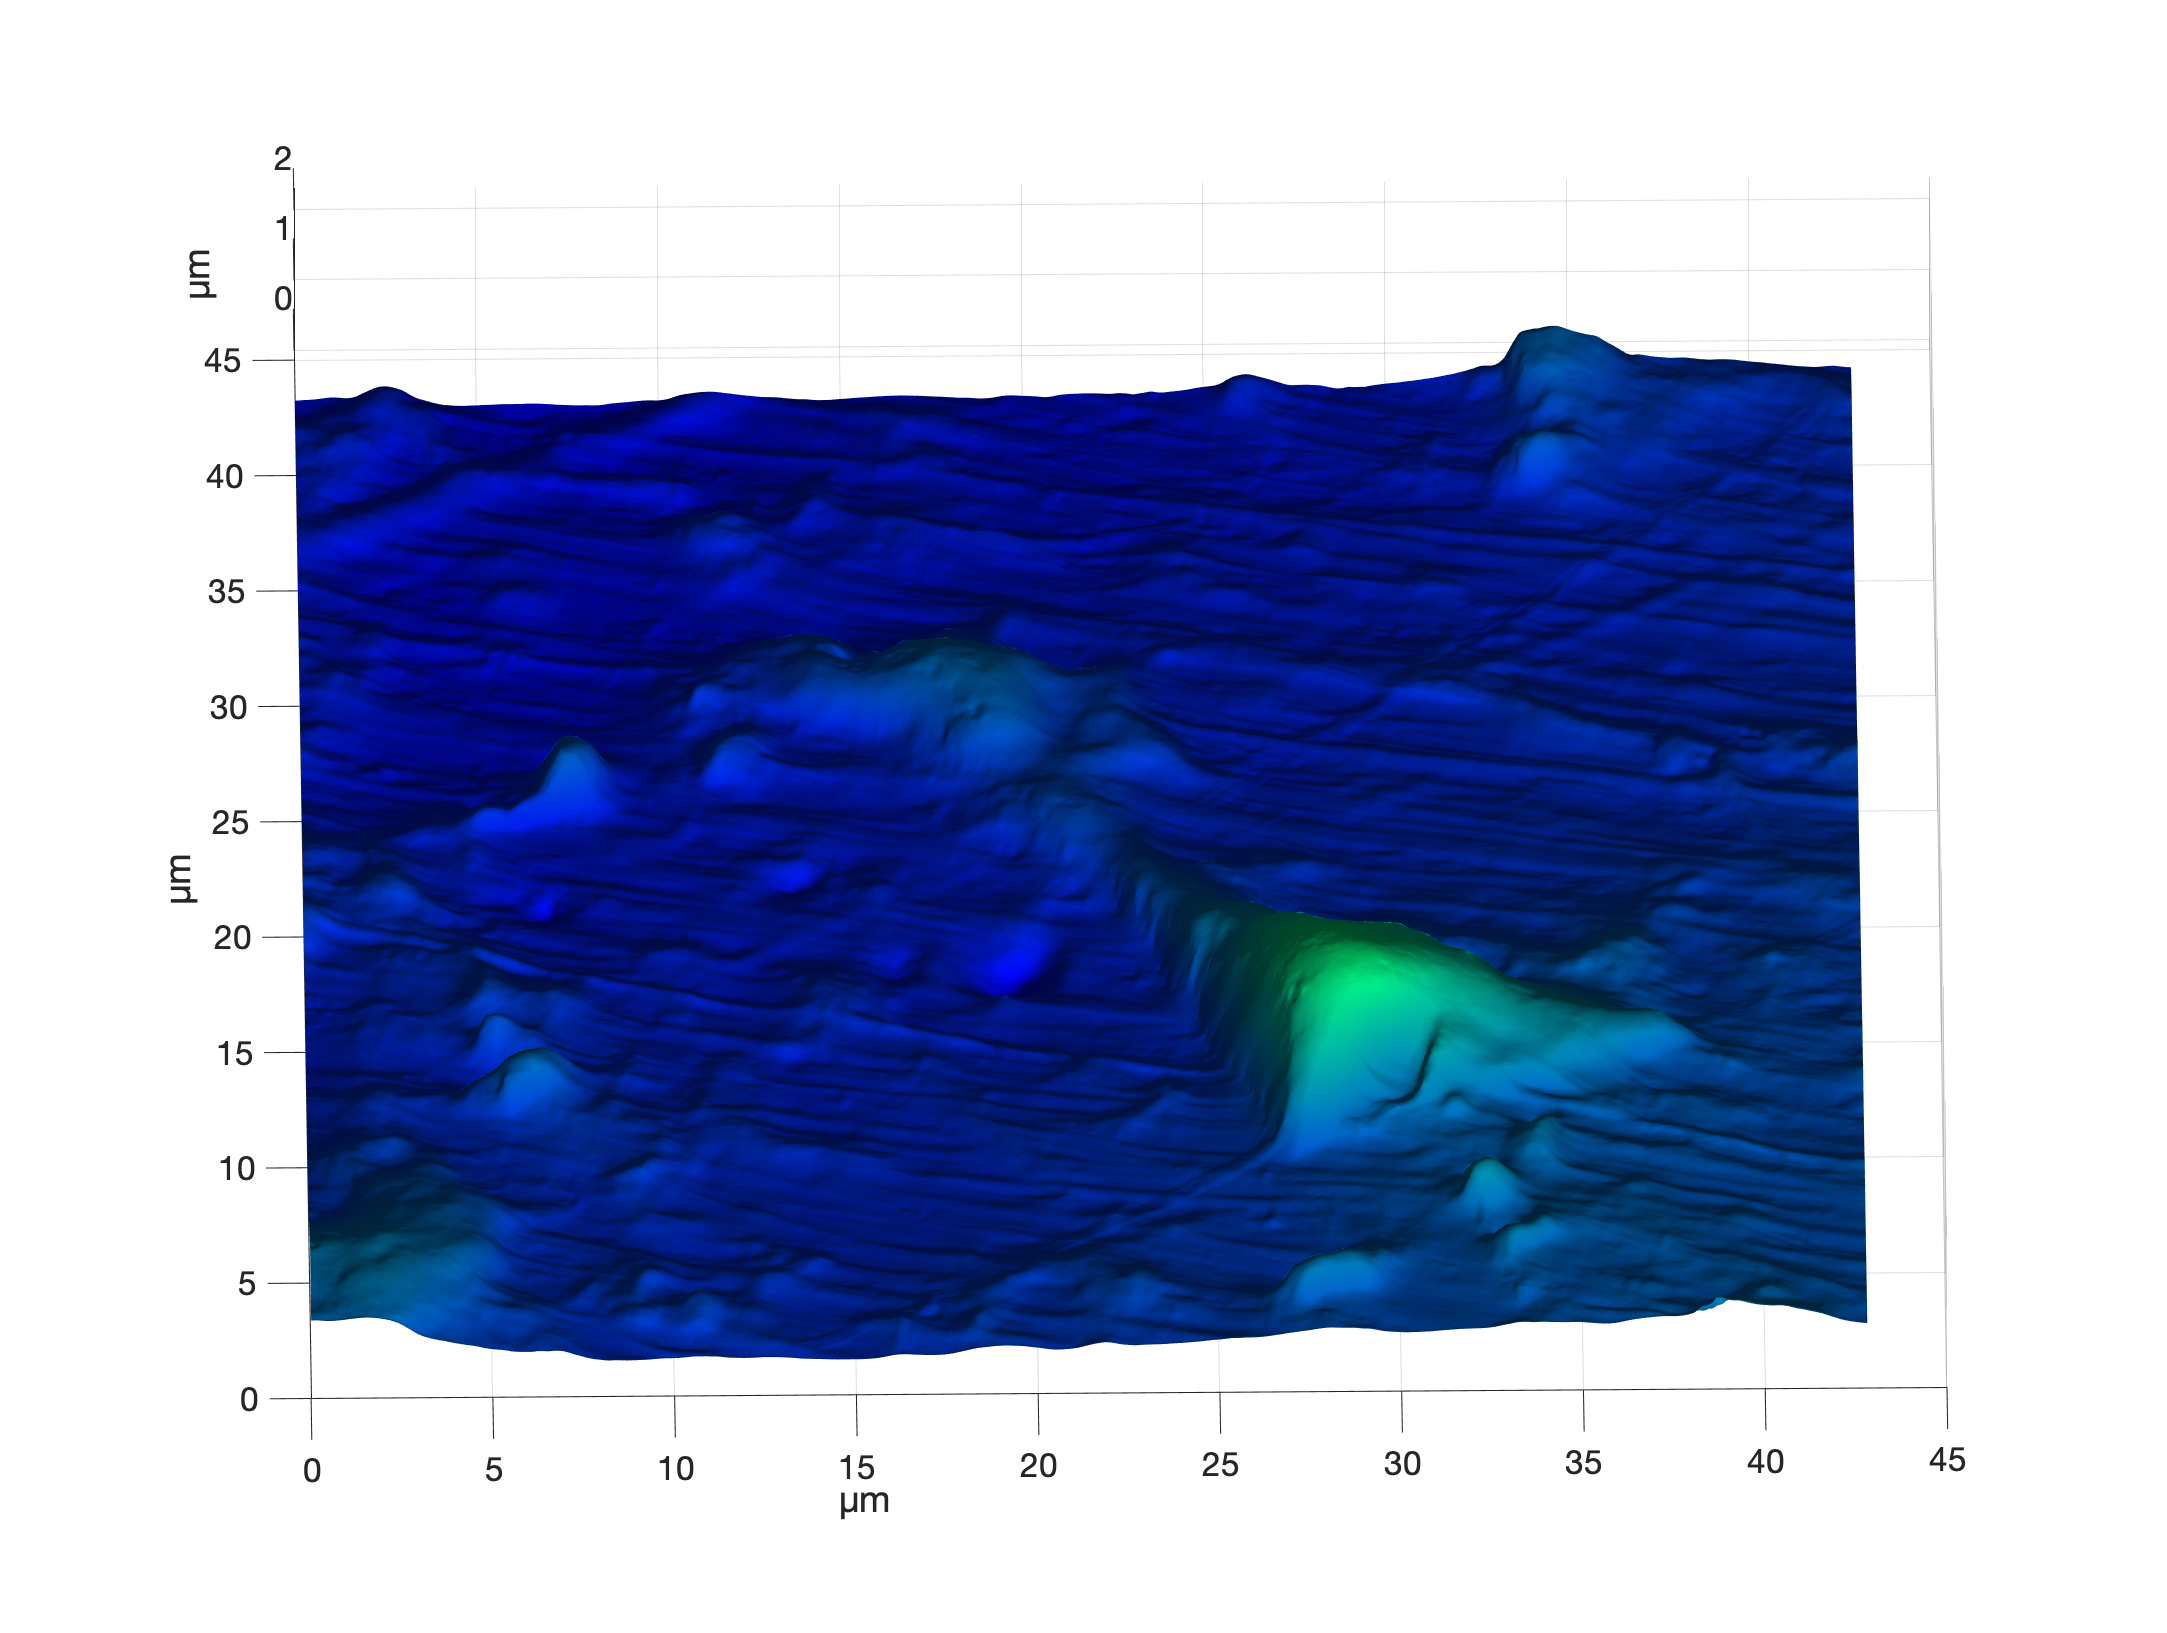
\includegraphics[width=1.0\linewidth]{tin-copper.eps}
        \end{column}
    \end{columns}
\end{frame}

\begin{frame}
    \frametitle{Экспериментальная установка}
    \begin{figure}
        \includegraphics[width=0.6\linewidth]{detector_structure.eps}
        \caption{Устройство детектора в плоскости $X$: $\alpha$~--- угол между нормалью малого
участка поверхности и электронным лучом $I_0$, $A,B,C,D$~--- детекторы, O-образец,
$\Omega_{b}$~--- телесный угол детектора $D$ отклоненного на угол $\theta_b$, $H$~--- рабочее
расстояние СЭМ.}
        {\label{fig:detector_structure}}% chktex 8
    \end{figure}
\end{frame}

\begin{frame}
    \frametitle{Постановка задачи}
    Согласно~\cite{PaluszynskiSlowko2005Vacuum, DrzazgaPaluszynski2005Measurement} интенсивность сигнала связана с углом наклона соответствующего участка поверхности:
    $$ I_{AB} = \frac{I_A - I_B}{I_A + I_B} \sim \tan{\alpha^x}, \quad I_{EF} = \frac{I_E - I_F}{I_E + I_F} \sim \tan{\alpha^y} $$
    \textbf{Задача 1:} Сигнал $I_{AB}(x,y), I_{EF}(x,y)$ в области $P$ предполагается известным. Необходимо восстановить градиент поверхности $\left(\frac{\partial Z}{\partial x}(x,y), \frac{\partial Z}{\partial y} (x,y) \right), (x,y) \in P$.

    \vfill

    \textbf{Задача 2:} Градиент
    \begin{equation}
        {\Big(\frac{\partial Z}{\partial x}(x,y),
        \frac{\partial Z}{\partial y} (x,y)\Big)}^{T} =
        {\big(P^x(x,y), P^y(x,y)\big)}^T, \quad (x,y) \in P
    \end{equation}
    предполагается известным. Найти функцию $Z(x,y)$ представляющую восстанавливаемую поверхность.
\end{frame}

%---------------------------------------------------------------------------------------------------

%---------------------------------------------------------------------------------------------------
\section{Восстановление градиента}
\begin{frame}
    \sectionpage
\end{frame}


\begin{frame}[c,allowframebreaks]
    \frametitle{Восстановление градиента}

    Применяя метод калибровочной поверхности (рис.~\ref{fig:inputSphere}), описанный в~\cite{main},
    необходимо восстановить аппаратные функции $F_x, F_y$ (рис~\ref{fig:Tables})).

    \begin{figure}[hp]
        \includegraphics[width=0.7\linewidth]{S.eps}
        \caption{\small Разностный сигнал $I_{AB}$ в направлении сканирования вдоль оси $x$~(a) и $y$~(b).}
        {\label{fig:inputSphere}}% chktex 8
    \end{figure}

    \framebreak

    Исследуемая область представляется в виде матриц $K^x$, $K^y$ размером $(N,N)$, элементами которых является интенсивность сигнала $k^x (i,j)$, $k^y (i,j)$ в точке $(x_j, y_i)$.

    Для каждого элемента $k^x_{i,j}$ матрицы $K^x$, который принадлежит калибровочной поверхности,
найдем производную $\frac{\partial z}{\partial x} \big|_{(x_j,y_i)} $ аналитически, таким
образом составляя таблицу, задающую сеточные значения функции обратной к аппаратной функции
$\hat{F^x}$ зависимости сигнала $K^x_{i,j} = F^x (\tan(\alpha^x_{i,j}))$ от угла наклона
поверхности $\alpha^x$ к оси $x$.
    \begin{center}
        \begin{tabular}{| c| c |}
            \hline
            $ k^x_{i,j} $ & $ \tan{ \frac{\partial z(x_j, y_i)}{\partial x} } $ \\
            \hline
            \vdots          & \vdots \\
            \hline
            $ k^x_{i',j'} $ & $ \tan{ \frac{\partial z(x_{j'}, y_{i'})}{\partial x} } $ \\
            \hline
        \end{tabular}
    \end{center}

    \framebreak

    \begin{figure}
        \includegraphics[width=0.9\linewidth]{Tables.eps}
        \caption{График аппаратных функций $F^x$, $F^y$ зависимости угла наклона поверхности (в градусах) от интенсивности сигнала. И их табличного представления $\hat{F^x}$, $\hat{F^y}$}
        {\label{fig:Tables}}% chktex 8
    \end{figure}

    \framebreak

    \begin{figure}
        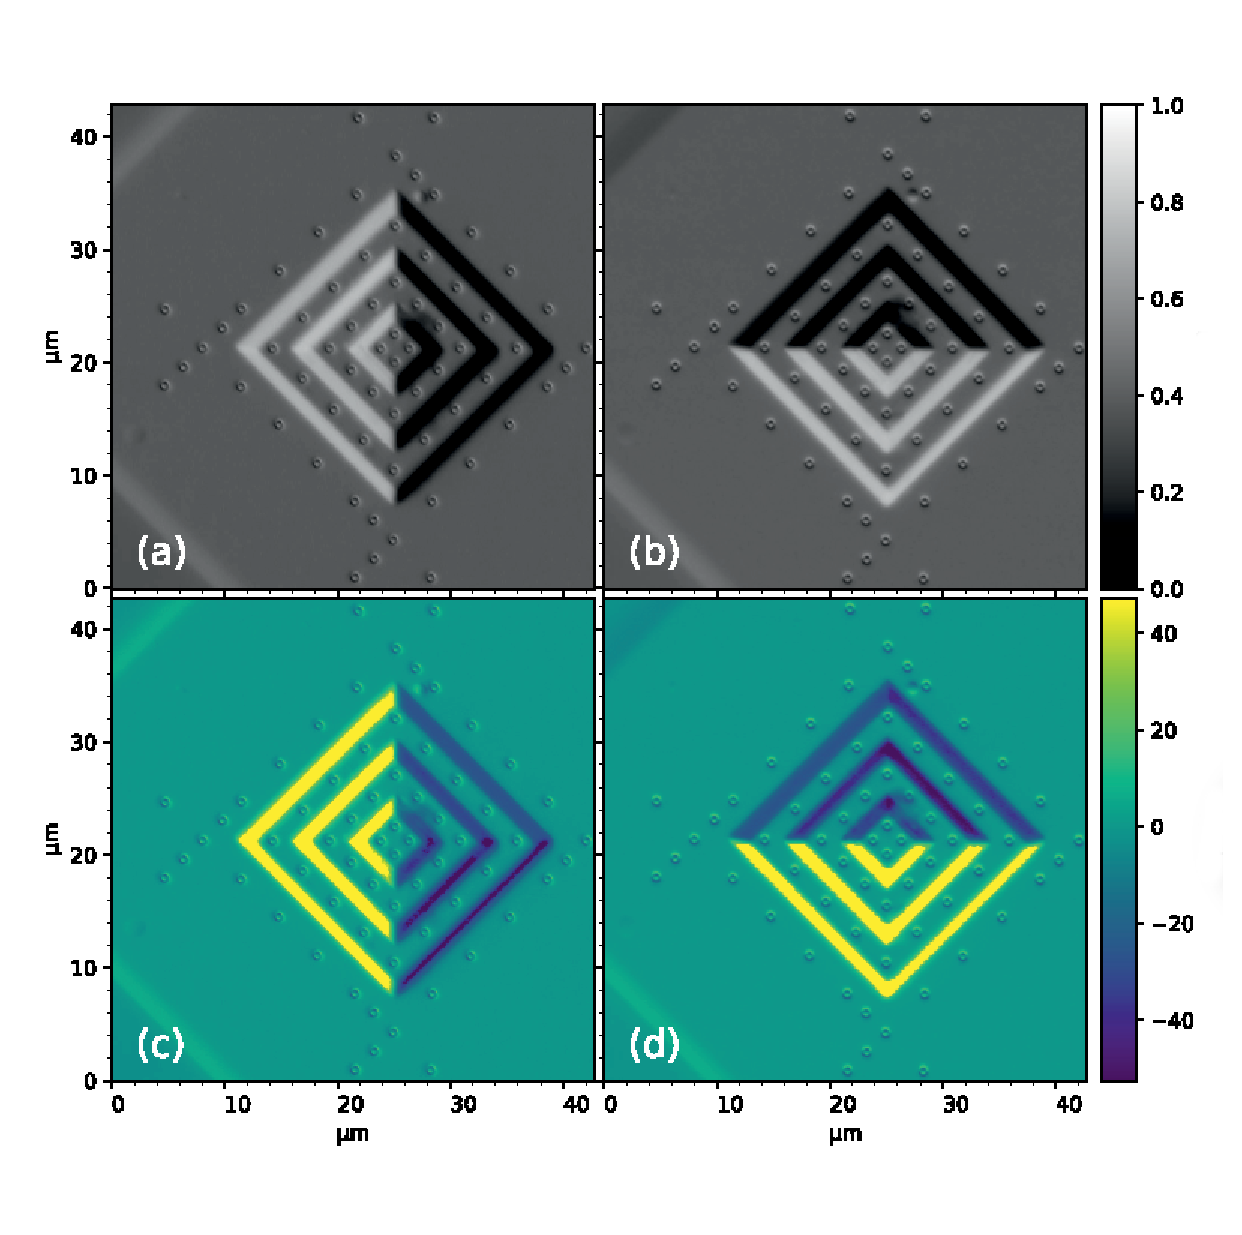
\includegraphics[width=0.5\linewidth]{P.eps}
        \caption{Входные изображения (a) и (b) восстанавливаемой поверхности и её карта углов (c) и (d).}
        {\label{fig:input_data}}% chktex 8
    \end{figure}
\end{frame}
% --------------------------------------------------------------------------------------------------


% --------------------------------------------------------------------------------------------------
% --------------------------------------------------------------------------------------------------
% --------------------------------------------------------------------------------------------------
\section{Восстановление поверхности}
\begin{frame}
    \sectionpage
\end{frame}


\begin{frame}[c,allowframebreaks]
    \frametitle{Восстановление поверхности}

    \begin{figure}
        \includegraphics[width=0.7\linewidth]{input_data2.eps}
        \caption{Different signals obtained with a scanning electron microscope in
$X$-direction~(a) and $Y$-direction~(b) to be reconstructed for a silver plate after
Vickers hardness . The blue line indicates the data source for the profilogram on
рис.~\ref{fig:results}.}
        {\label{fig:input_data2}}%
    \end{figure}

    Исходная задача~(\ref{problem_statement}) может быть сформулирована в операторном виде следующим образом
    \begin{equation*}
        \label{operator_equation_0}
        A[Z] = {\textbf{\emph{J}}},
    \end{equation*}
где оператор $A: W_2^2(S) \to L_2(S)$ непрерывен. Этот оператор связывает искомую функцию  is continuous and unique. This operator associates
    the function $Z(x,y)$ determining 3D surface of the sample with the gradient of the surface
    ${\textbf{\emph{J}}}$. Suppose that instead of accurately known $\bar{{\textbf{\emph{J}}}}$
    its approximate values ${\textbf{\emph{J}}}_\delta$ is known, such that
    $\|{\textbf{\emph{J}}}_\delta-\bar{{\textbf{\emph{J}}}}\|_{L_2}\leq\delta$. Typical experimental
    values of a signal which depends on the partial derivatives of the surface for fixed value $y$
    (blue line on рис.~\ref{fig:input_data2}) are represented on subfigure on рис.~\ref{fig:results}.

    \begin{figure}[t]
        \includegraphics[width=0.50\linewidth]{results.eps}
        \caption{The reconstructed surface whose input signal is shown on  рис.~\ref{fig:input_data}.}
        {\label{fig:results}}
    \end{figure}

    As a result, the inverse problem of reconstruction of 3D surface takes the form
    \begin{equation}
        \label{operator_equation}
        A[Z_\delta] = {\textbf{\emph{J}}}_\delta, \quad {\textbf{\emph{J}}}_\delta \in L_2(S).
    \end{equation}


    The solution to the inverse problem~(\ref{operator_equation}) can be found as an element $Z_\delta \in W_2^2(S)$ that realizes a minimum of the functional
    \begin{equation}
        \label{functional}
        F[Z] = \big\|A[Z] - {\textbf{\emph{J}}}_\delta\big\|_{L_2}^2.
    \end{equation}
\end{frame}
% --------------------------------------------------------------------------------------------------
% --------------------------------------------------------------------------------------------------
% --------------------------------------------------------------------------------------------------




% --------------------------------------------------------------------------------------------------
% --------------------------- N U M E R I C A L   R E A L I Z A T I O N ----------------------------
% --------------------------------------------------------------------------------------------------
\section{Численная реализация}
\begin{frame}
    \sectionpage
\end{frame}

\begin{frame}[c,allowframebreaks]
    \frametitle{Numerical realization}

    Input data ((a) and (b) at рис.~\ref{fig:input_data}) is represented as matrices $K^x$, $K^y$
    with sizes $(N \times N)$, their represent the signal intensities $k^x_{i,j} \equiv K^x (i,j)$,
    $K^y_{i,j} \equiv k^y (i,j)$ at points $(x_j, y_i) \in S$, $i,j = \overline{1,N}$, their values
    are normed at $1$. Applying the method of calibrating surface, described in~\cite{main},
    we obtain the components $J_x$ and $J_y$ of the gradient ${\textbf{\emph{J}}}$: $j^x_{i,j}$,
    $k^y_{i,j}$ at points $(x_j, y_i) \in S$, $i,j = \overline{1,N}$.
    The distance between two neighboring points along each of the coordinate axes is constant.

    To reconstruct surface topography we rewrite the equation~(\ref{operator_equation}) as
    $$ \nabla Z(x,y) = (J_x, J_y)^T, \quad (x,y)\in S,$$
    and add an initial condition $Z(x_0,y_0) = 0$, which is chosen arbitrarily for any point
    $(x_0,y_0) \in S$ (it is convenient to use $(x_0,y_0) \equiv (0,0)$).

    \framebreak

    Thus, the following problem should be solved:
    \begin{equation}
        \label{system_of_equations}
        \left\{
            \begin{aligned}
                &\nabla Z(x,y) = (J_x, J_y)^T, \quad (x,y)\in S, \\
                &Z(x_0,y_0) = 0.
            \end{aligned}
        \right.
    \end{equation}

    \framebreak

    Transform observed values of $J_x$ as follows:
    \begin{equation}
        \label{column-major_ordering}
        J_x \equiv
        \left(
            \begin{array}{cccc}
                j^x_{1,1} & j^x_{1,2} & \cdots & j^x_{1,N} \\
                j^x_{2,1} & j^x_{2,2} & \cdots & j^x_{2,N} \\
                \vdots & \vdots & \ddots & \vdots  \\
                j^x_{N,1} & j^x_{N,2} & \cdots & j^x_{N,N}
            \end{array}
        \right)
        \sim
        \left(
            \begin{array}{c}
                j^x_{1,1} \\
                j^x_{2,1} \\
                \vdots \\
                j^x_{N,1} \\
                j^x_{1,2} \\
                j^x_{2,2} \\
                \vdots \\
                j^x_{N,2} \\
                \vdots \\
                j^x_{1,N} \\
                \vdots \\
                j^x_{N,N}
            \end{array}
        \right)
        \equiv{}  B^x.
    \end{equation}
    Performing in a similar way with $J_y$ we obtain $B^y$, and with unknown surface $Z$ we obtain $\hat{Z}$.


    Thus the problem~(\ref{system_of_equations}) can be rewritten in the following matrix form:
    \begin{equation*}
        \label{matrix_equation}
        \hat{A} \hat{Z}  =
        \left(
        \begin{aligned}
            &B^x\\
            &B^y
        \end{aligned}
        \right)
        \equiv B.
    \end{equation*}
    Here matrix $\hat{A}$ with sizes $(2N^2 \times N^2)$ represents a finite difference
    approximation of operators $\frac{\partial}{\partial x}$ (first $N^2$ rows) and
    $\frac{\partial}{\partial y}$ (the last $N^2$ rows).

    \framebreak

    \small
    \begin{equation*}
        \begin{array}{lllll}
            a_{i,i}             & = &-1/h & for & i = \overline{1,N^2},                         \\
            a_{i,i+N}           & = &1/h  & for & i = \overline{1,N^2 - N},                     \\
            a_{i,i-N}           & = &1/h  & for & i = \overline{N^2 - N,N^2 },                  \\
            a_{N^2+i+j, i+j}    & = &-1/h & for & i = 1, N+1, 2N+1,~\dots, (N-1)N + 1,          \\
                                &   &       &   & j = \overline{0,N-2},                         \\
            a_{N^2+i+j, i+j+1}  & = &-1/h & for & i = 1, N+1, 2N+1,~\dots, (N-1)N + 1,          \\
                                &   &       &   & j = \overline{0,N-2},                         \\
            a_{N^2+i+N-1, i+N-1} &= &-1/h & for & i = 1, N+1, 2N+1,~\dots, (N-1)N + 1,          \\
            a_{N^2+i+N-1, i+N-2} &= &1/h  & for & i = 1, N+1, 2N+1,~\dots, (N-1)N + 1,
        \end{array}
    \end{equation*}
    where $h$ is a constant distance between two neighboring sample points along axis $X$ or $Y$.
    \normalsize

    \framebreak

    Its components are represented as
    where $h$ is a constant distance between two neighboring sample points along axis $X$ or $Y$.

    Then we find
    \begin{equation*}
        \hat{Z} = \operatorname{argmin}\limits_Z \|\hat{A} Z - B\|^2.
    \end{equation*}

\end{frame}
% --------------------------------------------------------------------------------------------------

% --------------------------------------------------------------------------------------------------
% -------------------------------- G A L L E R Y ---------------------------------------------------
% --------------------------------------------------------------------------------------------------
\section{Примеры восстановления поверхностей}
\begin{frame}
    \sectionpage
\end{frame}

\begin{frame}[c,allowframebreaks]
    \frametitle{Gallery}

    \begin{figure}
        \includegraphics[width=0.7\linewidth]{berger.eps}
        \caption{Reconstruction result of input data depicted in рис.~\ref{fig:input_data}.}
        {\label{fig:berger}}% chktex 8
    \end{figure}

\framebreak

    \begin{figure}
        \includegraphics[width=0.8\linewidth]{indentor-source.eps}
        \caption{Different signals obtained with a scanning electron microscope in $X$-direction~(a) and $Y$-direction~(b) to be reconstructed for a gold plate after Vickers hardness . The blue line indicates the data source for the profilogram on рис.~\ref{fig:indentor}.}
        {\label{fig:indentor-source}}% chktex 8
    \end{figure}

\framebreak

    \begin{figure}
        \includegraphics[width=0.5\linewidth]{indentor.eps}
        \caption{Reconstruction result of input data depicted in рис.~\ref{fig:indentor-source}.}
        {\label{fig:indentor}}% chktex 8
    \end{figure}

\end{frame}

\begin{frame}[c,allowframebreaks]
    \bibliography{bibliography}
\end{frame}

\begin{frame}[c]
    \frametitle{Thanks for attention!}
    Presentation source and text available through links:
    \url{https://github.com/aborzunov/20201201}
    \begin{figure}
        \includegraphics[width=0.5\linewidth]{repo_link.png}
    \end{figure}
    \usebeamerfont{institute} Contact: \url{Andrey.Borzunov@gmail.com}
\end{frame}

\end{document}
